\section{DVI decoder}

\subsection{\texttt{dvi2rgb} module overview}
\begin{figure}
  \centering
  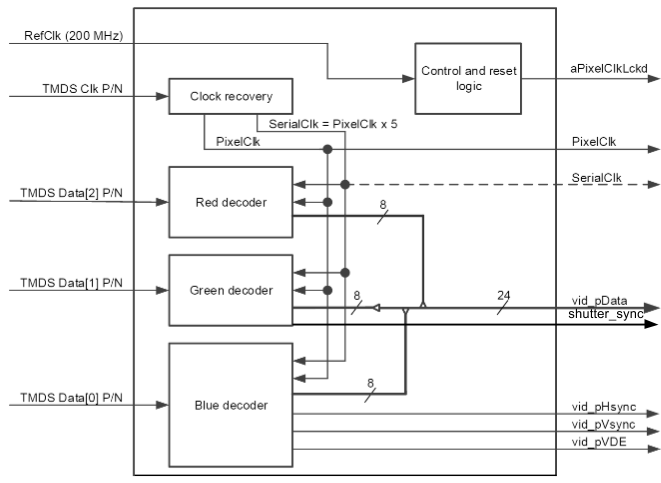
\includegraphics[width=1\textwidth]{./img/dvi2rgb.png}\par
  Source: \url{https://github.com/DigilentInc/vivado-library/blob/master/ip/dvi2rgb_v1_5/docs/dvi2rgb_v1_5.pdf}
  \caption{Block diagram of the DVI decoder.}
  \label{fig:dvi2rgb}
\end{figure}

The DVI decoder is connected via a \gls{hdmi} cable to the output of the DVI encoder on the sensor module board. It is important to note that the \gls{hdmi} port is connected directly to the \gls{fpga} and can be used to transmit anything provided the \gls{fpga} is configured correctly. The \gls{hdmi} ports have been carefully routed to carry four high-speed differential signals --- their controlled impedance makes them ideally suited to cope with the required bandwidth. As with the encoder, each channel is independent and so three identical decoders are instantiated, the output of which is concatenated to produce a 24-bit pixel bus accompanied by the standard video timing and synchronisation signals which are derived from the control data bits. In this proof-of-concept system the 8-bit pixel values from the OV7670 are tapped from the Blue channel on the receiver, a single control bit for the shutter synchronisation signal is tapped from the Green channel, and the Red channel remains unused.

\section{Clock recovery}
As the system is source-synchronous, the \gls{dvi} clock channel is used to drive the \gls{dvi} decoder logic on the receiver. The clock channel cannot be used directly, rather it contains a character-rate reference signal which is fed into a \gls{pll} to generate the pixel clock and serial clocks needed for the decoder logic to function. To generate these clocks an MMCME2\_ADV primitive, providing clock management functionality, is instantiated inside the \gls{dvi} decoder. Figure \ref{fig:clock_recovery} illustrates how the differential \gls{tmds} clock is fed into a differential input global clock buffer (\texttt{IBUFGDS}) connected to the input of the \gls{mmcm} primitive. The \gls{mmcm} contains a \gls{pll} clock multiplier which locks on to the reference clock and generates an output clock with a frequency five times higher. The output clock from the \gls{mmcm} is split and fed into two buffers. The first, a \texttt{BUFIO} primitive, provides the serial clock for the \texttt{ISERDESE2} primitives in the deserialisation logic. The second buffer is a \texttt{BUFR} primitive which has a frequency divider on it, which is used to divide the 5x serial clock back down and thus is how the pixel clock is generated. 

\begin{figure}
  \centering
  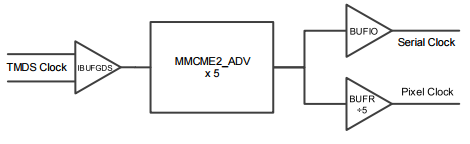
\includegraphics[width=1\textwidth]{./img/clock_recovery.png}\par
  Source: \url{https://github.com/DigilentInc/vivado-library/blob/master/ip/dvi2rgb_v1_5/docs/dvi2rgb_v1_5.pdf}
  \caption{Clock recovery overview.}
  \label{fig:clock_recovery}
\end{figure}

Inside the \gls{pll} a \gls{vco} is used is

\section{Deserialisation}

Phase alignment minimum freq
